\documentclass{article}

% Language setting
\usepackage[english]{babel}

% Set page size and margins
\usepackage[letterpaper,top=2cm,bottom=2cm,left=3cm,right=3cm,marginparwidth=1.75cm]{geometry}

% Useful packages
\usepackage{amsmath}
\usepackage{graphicx}
\usepackage[colorlinks=true, allcolors=blue]{hyperref}
\usepackage{float}
\DeclareMathOperator*{\argminA}{arg\,min}

\title{CS461 HW5}
\author{John Bailon}
\date{December 16, 2024}

\begin{document}
\maketitle

\noindent
Submission Files:

\section{EM Algorithm}
\subsection{Log-Likelihood}
\subsection{E-Step}
\subsection{M-Step}
\subsection{Updated Log-likelihood}

\section{Exact v. Approximate inference}
\subsection{Variable Elimination}
Using the structure of the provided network and conditional probability and marginalization we have,

\[ P(Cloudy | Sprinkler = T, WetGrass = T) = \alpha\sum_{rain} P(Cloudy, Sprinkler, Rain, Wet Grass)\]

We will use normalization later to find the posterior probability. Next, we substitute the joint probability for its bayesian network representation

\[ = \alpha \sum_{rain} P(Cloudy) * P(Sprinkler | Cloudy) * P(Rain | Cloudy) * P(WetGrass | Sprinkler, rain)\]

\[ = \alpha * P(Cloudy) * P(Sprinkler | Cloudy) \sum_{rain} P(Rain | Cloudy) * P(WetGrass | Sprinkler, rain)\]

For Cloudy = T

\[ = \alpha * 0.5 * 0.1 * ((0.8 * 0.99) + (0.2 * 0.9))\]
\[ = 0.0486\alpha\]

For Cloudy = F

\[ = \alpha * 0.5 * 0.5 * ((0.2 * 0.99) + (0.8 * 0.9))\]
\[ = 0.2295\alpha\]

Finally, normalize

\[P(Cloudy | Sprinkler = T, WetGrass = T) = \frac{0.0486}{0.0486 + 0.2295} = 17.48 \%\]

\subsection{Gibbs Sampling}
For Gibbs sampling, we will assign all variables in the network to arbitrary values, fixing the evidence variables, sprinkler, and wet grass, to true. Next, we will generate samples for both cloudy and rainy by calculating their probability conditional on their Markov blankets. The general form is

\[ P(Target | Markov Blanket) = \alpha P(Target | Parent) * P(Children | Coparent and Target)\]

For Cloudy:
\[ P(Cloudy | Sprinkler, Rainy) = \alpha P( Cloudy) * P(Sprinkler | Cloudy) * P(Rainy | Cloudy)\]

For Rainy:
\[ P(Rainy | Cloudy, wetgrass, Sprinkler) = \alpha P(Rainy | Cloudy) * P(WetGrass | Sprinkler, Rainy)\]

We will assign cloudy and rainy based on the computed probability and repeat. The mean of the generated sample will approximate the prior.

Below is the code I used to solve this problem. After 1,000,000 iterations, the prior is estimated to be 17.53\%.

\begin{figure}[H]
    \centering
    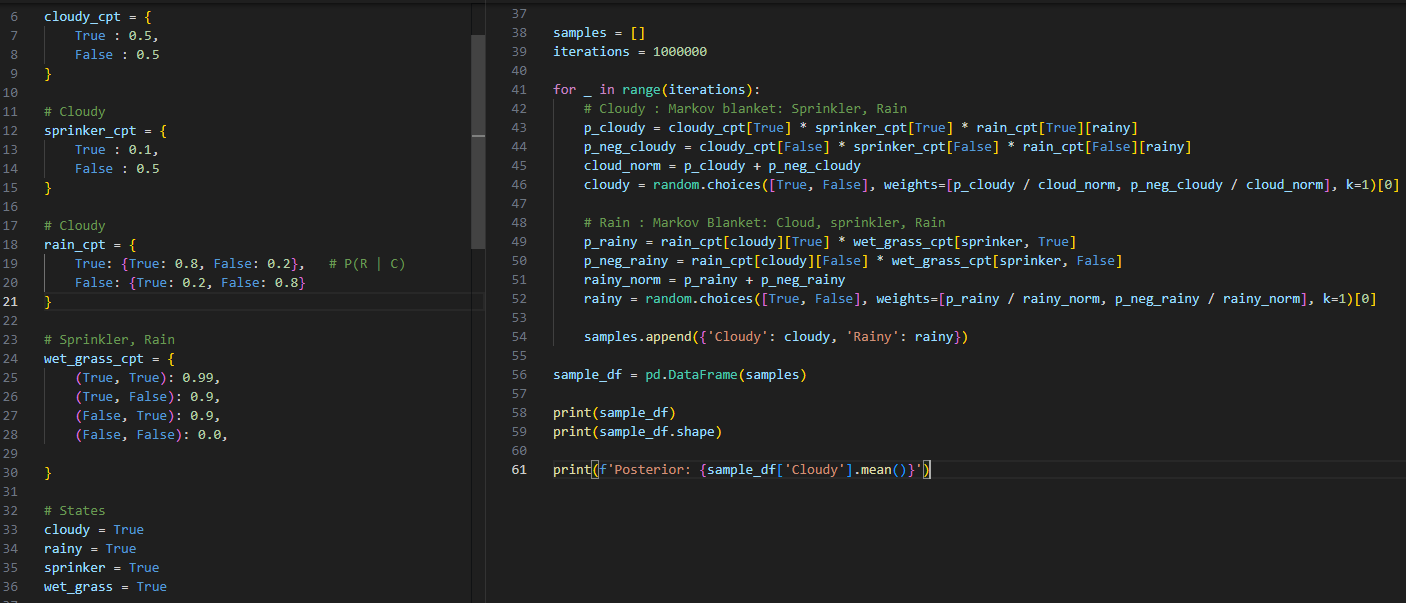
\includegraphics[width=1\linewidth]{Q2 Code.png}
    \caption{2.2 Gibbs Sampling Implementation}
    \label{fig:enter-label}
\end{figure}

\section{VAE Lower Bound (ELBO)}
\subsection{Derive the Inequality}

\section{RBM Movie Recommendation System}
\subsection{Bipolar Coding}
\subsection{Modify RBM}
\subsection{Predict Movie Preference}

\end{document}